% !TEX root = ../../report.tex

\section{Триггеры и хранимая функция}

В проектируемой базе данных предусмотрены два триггера и одна хранимая функция.

\subsection{Триггер аудита изменений цен}

Триггер \texttt{catch\_price\_change} активируется после обновления столбца \texttt{price} в таблице \texttt{products}. Условие срабатывания --- старое значение цены отличается от нового. При срабатывании вызывается функция аудита цены, которая вставляет запись в таблицу \texttt{product\_price\_history}, содержащую:

\begin{itemize}
    \item идентификатор товара;
    \item старую и новую цену;
    \item метку времени изменения;
    \item имя пользователя, инициировавшего изменение.
\end{itemize}

Схема алгоритма триггера приведена на рисунке~\ref{fig:trigger_price}.

\begin{figure}[H]
    \centering
    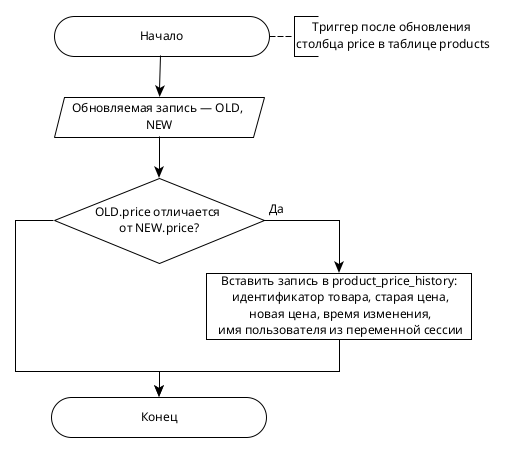
\includegraphics[width=0.7\textwidth]{img/trigger_catch_price_change.png}
    \caption{Схема алгоритма триггера аудита изменений цен}
    \label{fig:trigger_price}
\end{figure}

Триггер обеспечивает автоматическое формирование журнала изменения цен.

\subsection{Триггер пересчёта рейтингов}

Триггер \texttt{update\_ratings\_on\_review} активируется после вставки новой записи, обновления столбца \texttt{rating} или удаления записи в таблице \texttt{reviews}. Вызываемая функция \texttt{update\_product\_and\_seller\_rating} выполняет каскадный пересчёт:

\begin{enumerate}
    \item определяется идентификатор затронутого товара;
    \item рейтинг товара обновляется как среднее арифметическое оценок всех отзывов на данный товар (\texttt{AVG(rating)});
    \item по идентификатору продавца, полученному из обновлённой записи товара, пересчитывается рейтинг продавца как среднее арифметическое рейтингов всех его неудалённых товаров, имеющих хотя бы один отзыв.
\end{enumerate}

Схема алгоритма триггера приведена на рисунке~\ref{fig:trigger_rating}.

\begin{figure}[H]
    \centering
    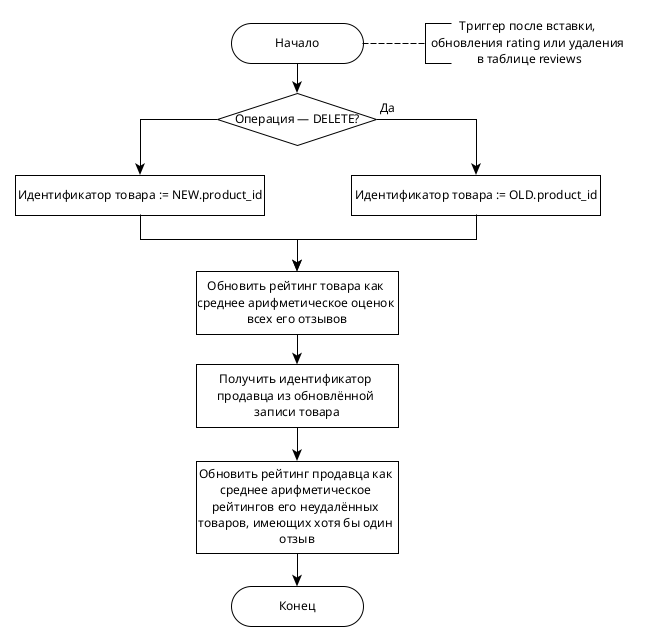
\includegraphics[width=0.7\textwidth]{img/trigger_update_ratings_on_review.png}
    \caption{Схема алгоритма триггера пересчёта рейтингов}
    \label{fig:trigger_rating}
\end{figure}

Такой подход поддерживает согласованность рейтингов: при добавлении, изменении или удалении отзыва автоматически обновляются рейтинги товара и продавца.

\subsection{Хранимая функция статистики продавца}

Функция \texttt{get\_seller\_statistics} принимает три параметра: идентификатор продавца (\texttt{p\_seller\_id}), начальную (\texttt{p\_date\_from}) и конечную (\texttt{p\_date\_to}) даты периода. Возвращает таблицу из четырёх столбцов:

\begin{itemize}
    \item \texttt{total\_orders} --- количество уникальных заказов;
    \item \texttt{total\_revenue} --- суммарная выручка;
    \item \texttt{avg\_order\_value} --- средний чек;
    \item \texttt{top\_product\_name} --- наименование самого продаваемого товара по количеству проданных единиц.
\end{itemize}

Функция объединяет данные таблиц \texttt{orders}, \texttt{order\_items} и \texttt{products} по идентификатору продавца и заданному временному интервалу. В расчёт включаются только заказы со статусами \texttt{paid}, \texttt{shipped} и \texttt{delivered}, что исключает из статистики неоплаченные и отменённые заказы.

Выручка рассчитывается как сумма произведений количества единиц товара на цену в момент покупки, что обеспечивает корректность подсчёта при наличии изменений цен. Средний чек вычисляется путём деления выручки на количество уникальных заказов.

Схема алгоритма функции приведена на рисунке~\ref{fig:function_stats}.

\begin{figure}[H]
    \centering
    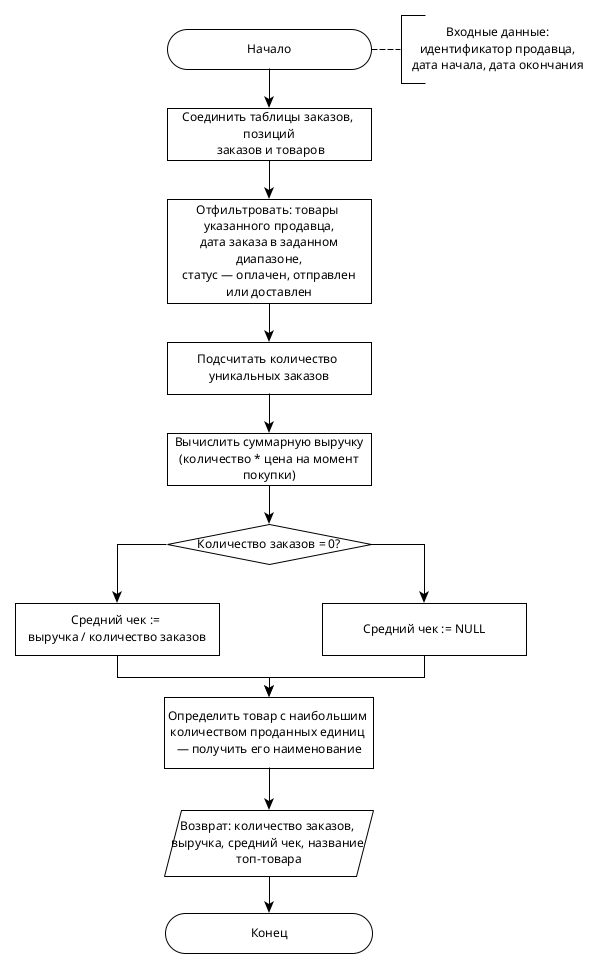
\includegraphics[width=0.7\textwidth]{img/function_get_seller_statistics.png}
    \caption{Схема алгоритма хранимой функции статистики продавца}
    \label{fig:function_stats}
\end{figure}
